\chapter{Modelli}
\section{Automi cellulari}
Gli automi cellulari possono riprodurre fenomeni di auto-riproduzione e
auto-organizzazione, sono utili per modellare sistemi complessi dinamici e la
simulazione. Utili per simulare e studiare sistemi come: traffico, afflusso di
persone, percolazione (studio della fluido dinamica), sistema immunitario, sistemi
sociali etc\dots.

L'idea è di non descrivere il sistema complesso dall'alto, ad alto livello usando
sistemi di equazione differenziali. In realtà lo si fa simulando l'interazione
tra le celle, ognuna delle quali è definita attraverso una serie di regole locali
semplici.

Gli automi cellulari sono dei sistemi dinamici e discreti, dove i termini
rappresentano:
\begin{itemize}
    \item \textbf{Sistemi}: insieme di entità che interagiscono.
    \item \textbf{Dinamici}: evolvono nel tempo in un insieme di passi.
    \item \textbf{Discreti}: spazio, tempo e proprietà devono essere solo finiti
          con un numero numerabile di stati. Spazio finito perché dobbiamo
          rappresentare la realtà.
\end{itemize}
Esistono automi cellulari a più dimensioni che specificano quante dimensioni è lo
spazio.

Lo spazio su cui essi operano è rappresentato da una griglia di celle discrete.
Inoltre, si ha un tempo di evoluzione discreto.

Lo stato che ogni cella assume è definito a partire da un insieme finito di stati
possibili. Inoltre, l'evoluzione di ogni cella è determinata da una regola comune
per tutte le celle, e dipende solamente dallo stato attuale della cella e dagli
stati dei suoi vicini. La regola di aggiornamento è quindi locale e uniforme.
\begin{definizione}[\textbf{Automa cellulare}]
    Un \textbf{automa cellulare} è definito come una tupla:
    \begin{equation*}
        \langle L, Q, q_0, u,f\rangle
    \end{equation*}
    dove:
    \begin{itemize}
        \item $L$: è l'array di automi a stati finiti uniformi.
        \item $Q$: insieme di stati finiti.
        \item $q_0$: è lo stato iniziale.
        \item $u$: è una funzione che definisce il criterio di connessione della
              singola cella con quelle adiacenti.
              \begin{equation*}
                  u: L \rightarrow L^{k}
              \end{equation*}
        \item $f$: la regola di transizione locale.
              \begin{equation*}
                  f: Q^{k} \rightarrow Q
              \end{equation*}
    \end{itemize}
\end{definizione}
Lavorando con automi cellulari finiti, ovvero con lo spazio finito, sarà
importante definire una \textbf{condizione di bordo}, ovvero come deve essere la
regola del vicinato quando le celle sono vicino al bordo. La scelta della
condizione di bordo può essere fatta in questo modo:
\begin{itemize}
    \item Collegare i bordi: i bordi opposti dello spazio sono collegati. Si crea
          quindi un ambiente toroidale.
    \item Guardare i bordi come uno specchio: si considera che il bordo sia uno
          specchio, quindi si riflette il contenuto della cella.
\end{itemize}
Per gli automi cellulari 1-D in cui gli stati delle celle sono binari, si possono
codificare le regole attraverso numeri decimali.

Per mostrare l'evoluzione dell'automa 1D si usa il diagramma spazio-tempo, dove
si mostra l'evoluzione dell'automa nel tempo.
\begin{esempio}[Traffico]
    La regola del traffico è rappresentata dal valore 184. Essa permette di
    modellare semplicemente il flusso del traffico su una strada a singola corsia.

    La rappresentazione del traffico avviene nel seguente modo:
    \begin{figure}[!ht]
        \centering
        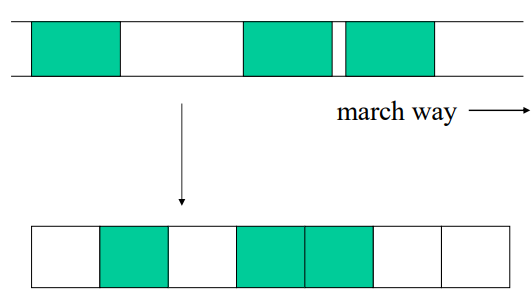
\includegraphics[width=0.5\textwidth]{./img/modelli/ese_traffico.png}
        \caption{Esempio di automa cellulare per la rappresentazione del traffico.}
        \label{fig:ese_traffico}
    \end{figure}
    La regola 184 è definita come segue:
    \begin{itemize}
        \item 111: il veicolo rimane fermo (1)
        \item 110: il veicolo si sposta in avanti e quindi la cella rimane vuota
              (0)
        \item 101: la cella è vuota e quindi il veicolo a sinistra si sposta
              occupando la cella (1)
        \item 100: la cella è vuota e quindi il veicolo a sinistra si sposta
              occupando la cella (1)
        \item 011: la cella a destra è occupata quindi il veicolo rimane fermo
              (1)
        \item 010: la cella a destra è vuota e quindi il veicolo si sposta in
              avanti (0)
        \item 001: non ci sono veicoli nella cella attuale e nella precedente
              quindi resta vuota (0)
        \item 000: non ci sono veicoli la cella è vuota (0)
    \end{itemize}

    Questo modello non rappresenta la realtà, in quanto ogni macchina si muove a
    step di 1 se c'è spazio, altrimenti si ferma. Inoltre, non si considera il
    tempo di reazione del guidatore e molti altri fattori.

    Possiamo complicare leggermente il modello sostituendo il valore che 
    rappresenta la presenza o meno del veicolo con la velocità del veicolo.
    Si aumenta il raggio delle celle da considerare come vicine. Inoltre, ogni 
    veicolo accelera di una velocità fino a quando non rischia di fare incidenti.
\end{esempio}
